\documentclass[epsfig,a4paper,11pt,titlepage,oneside,openany]{book}
\usepackage{epsfig}
\usepackage{plain}
\usepackage{setspace}
\usepackage[paperheight=29.7cm,paperwidth=21cm,outer=1.5cm,inner=2.5cm,top=2cm,bottom=2cm]{geometry}
\usepackage{titlesec} % per formato custom dei titoli dei capitoli

\usepackage{hyperref}
\usepackage{listings}

\usepackage{graphicx}
\graphicspath{ {./images/} }

\begin{document}


\pagenumbering{gobble}

% Pagina iniziale
\pagestyle{plain}

\thispagestyle{empty}

\begin{center}
  \begin{figure}[h!]
    \centerline{
\psfig{file=marchio_unitrento_colore_it_202002.eps,width=0.6\textwidth}}
  \end{figure}

  \vspace{2 cm} 

  \LARGE{Department of Information Engineering and Computer Science\\}

  \vspace{1 cm} 
  \Large{NETWORK SECURITY\\LABORATORY REPORT}

  \vspace{2 cm} 
  \vspace{1 cm} 
  \Huge\textsc{LAB 10\\HONEYPOT}


  \vspace{2 cm} 
  \begin{tabular*}{\textwidth}{ c @{\extracolsep{\fill}} c }
  \Large{Da Rold Giovanni}& \Large{Meschini Marcello}\\
  \Large{224291}& \Large{220222}\\
  \end{tabular*}

  \vspace{2 cm} 

  \Large{Academic year 2020/2021}
  
\end{center}
\clearpage

\pagestyle{plain}
\mainmatter
% indice
\tableofcontents
\clearpage
    
    
          
% gruppo per definizone di successione capitoli senza interruzione di pagina
\begingroup
% nessuna interruzione di pagina tra capitoli
% ridefinizione dei comandi di clear page
\renewcommand{\cleardoublepage}{} 
\renewcommand{\clearpage}{} 
\titleformat{\chapter}
  {\normalfont\Huge\bfseries}{\thechapter}{1em}{}
  
\titlespacing*{\chapter}{0pt}{0.59in}{0.02in}
\titlespacing*{\section}{0pt}{0.20in}{0.02in}
\titlespacing*{\subsection}{0pt}{0.10in}{0.02in}

\chapter*{Info about the lab} % senza numerazione
\label{info}

\addcontentsline{toc}{chapter}{Info about the lab} % da aggiungere comunque all'indice
\section*{Requirements}
\begin{itemize}
\item Docker Engine version 17.05 or newer
\item Docker Compose version 1.20.0 or newer
\item 2 GB of RAM
\item At least 20 GB of disk
\end{itemize}

\section*{Network Topology}
To create a network for the laboratory we used Docker Compose and created the following topology:
\begin{center}
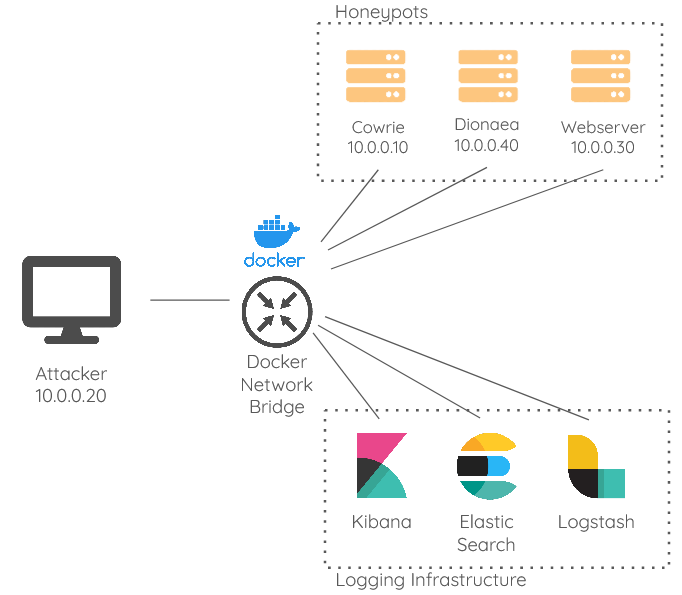
\includegraphics[scale=0.25]{topology}
\end{center}
The docker-compose.yaml file containing the definition for the containers can be found in the netsec-honeypot-lab folder on the desktop or in our Github public repository: 

\url{https://github.com/Marcy-P/netsec-honeypot-lab}

\noindent The repository README also contains additional info for accessing the containers and the references to some Docker images we used.

\section*{Starting up the lab}
To start the laboratory login into the VM with the credentials: username: \textit{netsec} and password: \textit{password}. Then open a terminal in the folder \textbackslash netsec-honeypot-lab on the desktop and type the following command:

\begin{lstlisting}[language=bash]
$ ./start.sh
\end{lstlisting}

\section*{Shutting down the lab}
To shut down the docker-compose network type:

\begin{lstlisting}[language=bash]
$ docker-compose down
\end{lstlisting}

\noindent To also clean the persistent data present in Elasticsearch type:

\begin{lstlisting}[language=bash]
$ docker-compose down -v
\end{lstlisting}

\chapter{What is a honeypot?}
\label{cha:intro}

"A honeypot is a network-attached system set up as a decoy to lure cyber attackers and detect, deflect and study hacking attempts to gain unauthorized access to information systems"\cite{coulouris}. So it is a system that is unprotected and serves no business purpose but sits in the network waiting to be contacted. Every interaction with a honeypot is suspicious because no legitimate user should utilize it.

\chapter{Characteristics of a honeypot}
\label{cha:characteristics}

Honeypots have four main characteristics; they have to be:
\begin{enumerate}
\item Deceptive
\item Discoverable
\item Interactive
\item Monitored
\end{enumerate}

\section{Deception}
\section{Discoverability}
\section{Interactivity}
\section{Monitoring}

\endgroup


% bibliografia in formato bibtex
%
% aggiunta del capitolo nell'indice
\addcontentsline{toc}{chapter}{Bibliography}
% stile con ordinamento alfabetico in funzione degli autori
\bibliographystyle{plain}
\bibliography{biblio}
\end{document}